\RequirePackage{atbegshi}
\documentclass[compress,aspectratio=169]{beamer}\usepackage[]{graphicx}\usepackage[]{color}
% maxwidth is the original width if it is less than linewidth
% otherwise use linewidth (to make sure the graphics do not exceed the margin)
\makeatletter
\def\maxwidth{ %
  \ifdim\Gin@nat@width>\linewidth
    \linewidth
  \else
    \Gin@nat@width
  \fi
}
\makeatother

\definecolor{fgcolor}{rgb}{0.345, 0.345, 0.345}
\makeatletter
\@ifundefined{AddToHook}{}{\AddToHook{package/xcolor/after}{\definecolor{fgcolor}{rgb}{0.345, 0.345, 0.345}}}
\makeatother
\newcommand{\hlnum}[1]{\textcolor[rgb]{0.686,0.059,0.569}{#1}}%
\newcommand{\hlstr}[1]{\textcolor[rgb]{0.192,0.494,0.8}{#1}}%
\newcommand{\hlcom}[1]{\textcolor[rgb]{0.678,0.584,0.686}{\textit{#1}}}%
\newcommand{\hlopt}[1]{\textcolor[rgb]{0,0,0}{#1}}%
\newcommand{\hlstd}[1]{\textcolor[rgb]{0.345,0.345,0.345}{#1}}%
\newcommand{\hlkwa}[1]{\textcolor[rgb]{0.161,0.373,0.58}{\textbf{#1}}}%
\newcommand{\hlkwb}[1]{\textcolor[rgb]{0.69,0.353,0.396}{#1}}%
\newcommand{\hlkwc}[1]{\textcolor[rgb]{0.333,0.667,0.333}{#1}}%
\newcommand{\hlkwd}[1]{\textcolor[rgb]{0.737,0.353,0.396}{\textbf{#1}}}%
\let\hlipl\hlkwb

\usepackage{framed}
\makeatletter
\newenvironment{kframe}{%
 \def\at@end@of@kframe{}%
 \ifinner\ifhmode%
  \def\at@end@of@kframe{\end{minipage}}%
  \begin{minipage}{\columnwidth}%
 \fi\fi%
 \def\FrameCommand##1{\hskip\@totalleftmargin \hskip-\fboxsep
 \colorbox{shadecolor}{##1}\hskip-\fboxsep
     % There is no \\@totalrightmargin, so:
     \hskip-\linewidth \hskip-\@totalleftmargin \hskip\columnwidth}%
 \MakeFramed {\advance\hsize-\width
   \@totalleftmargin\z@ \linewidth\hsize
   \@setminipage}}%
 {\par\unskip\endMakeFramed%
 \at@end@of@kframe}
\makeatother

\definecolor{shadecolor}{rgb}{.97, .97, .97}
\definecolor{messagecolor}{rgb}{0, 0, 0}
\definecolor{warningcolor}{rgb}{1, 0, 1}
\definecolor{errorcolor}{rgb}{1, 0, 0}
\makeatletter
\@ifundefined{AddToHook}{}{\AddToHook{package/xcolor/after}{
\definecolor{shadecolor}{rgb}{.97, .97, .97}
\definecolor{messagecolor}{rgb}{0, 0, 0}
\definecolor{warningcolor}{rgb}{1, 0, 1}
\definecolor{errorcolor}{rgb}{1, 0, 0}
}}
\makeatother
\newenvironment{knitrout}{}{} % an empty environment to be redefined in TeX

\usepackage{alltt} % aspectratio=169


% % % % % % % % % % % % % % %
%             MY PACKAGES 
% % % % % % % % % % % % % % %
\usepackage{graphicx}       % Use pdf, png, jpg, or eps with pdflatex; use eps in DVI mode
\usepackage{dcolumn} % this pack is neccesary to build nicer columns with texreg--dont remove it.
\usepackage[export]{adjustbox}
\usepackage{xcolor}[dvipsnames]
\usepackage{amssymb,amsmath}
\usepackage{threeparttable} % package to have long notes in reg tables in texreg. 
\usepackage{graphics}
\usepackage{pgfplots}
\pgfplotsset{compat=1.11}
\usepgfplotslibrary{fillbetween}

%\usepackage{tipx}
%\usepackage{tikz}
%\usetikzlibrary{arrows,shapes,decorations.pathmorphing,backgrounds,positioning,fit,petri}
\usepackage{rotating}
%\usepackage{scalerel} % for inline images
\usepackage{import}
%\usepackage{times}
\usepackage{array}
\usepackage{tabularx}
\usepackage{booktabs}
%\usepackage{textcomp}
\usepackage{float}
%\usepackage{setspace}      % \doublespacing \singlespacing \onehalfspacing %doble espacio
%\label{x:y}                          %ocupar para autoref.
%\autoref{x:y}                        %ocupar para autoref.
%\usepackage{nopageno}      %desactivar para p�ginas
\usepackage{pifont}
\newcommand{\xmark}{\ding{55}}%

%\usepackage{marvosym} %faces
\usepackage{hyperref}
\usepackage{multirow}

\usepackage{tikz}
\usetikzlibrary{arrows,decorations.pathreplacing}



\usepackage{listings}
\usepackage{color}
\definecolor{dkgreen}{rgb}{0,0.6,0}
\definecolor{gray}{rgb}{0.5,0.5,0.5}
\definecolor{mauve}{rgb}{0.58,0,0.82}
\lstset{ %
  language=R,                     % the language of the code
  basicstyle=\TINY,           % the size of the fonts that are used for the code
  numbers=left,                   % where to put the line-numbers
  numberstyle=\tiny\color{gray},  % the style that is used for the line-numbers
  stepnumber=1,                   % the step between two line-numbers. If it's 1, each line
                                  % will be numbered
  numbersep=5pt,                  % how far the line-numbers are from the code
  backgroundcolor=\color{white},  % choose the background color. You must add \usepackage{color}
  showspaces=false,               % show spaces adding particular underscores
  showstringspaces=false,         % underline spaces within strings
  showtabs=false,                 % show tabs within strings adding particular underscores
  frame=single,                   % adds a frame around the code
  rulecolor=\color{black},        % if not set, the frame-color may be changed on line-breaks within not-black text (e.g. commens (green here))
  tabsize=1,                      % sets default tabsize to 2 spaces
  captionpos=b,                   % sets the caption-position to bottom
  breaklines=true,                % sets automatic line breaking
  breakatwhitespace=false,        % sets if automatic breaks should only happen at whitespace
  title=\lstname,                 % show the filename of files included with \lstinputlisting;
                                  % also try caption instead of title
  keywordstyle=\color{blue},      % keyword style
  commentstyle=\color{dkgreen},   % comment style
  stringstyle=\color{mauve},      % string literal style
  escapeinside={\%*}{*)},         % if you want to add a comment within your code
  morekeywords={*,...}            % if you want to add more keywords to the set
} 

% % % % % % % % % % % % % % %
%           PACKAGE CUSTOMIZATION
% % % % % % % % % % % % % % %

% GENERAL CUSTOMIZATION
\usepackage[math]{iwona}% font
\usetheme{Singapore}  % template I should use
%\usetheme{Szeged}  % alternative template
\usecolortheme{rose}  % color template
\makeatletter     % to show subsection/section title (1/3)
\beamer@theme@subsectiontrue % to show subsection/section title (2/3)
\makeatother      % to show subsection/section title (3/3)



% THIS BELOW IS TO MAKE NAVIGATION DOTS MARKED DURING PRESENTATION
\makeatletter
\def\slideentry#1#2#3#4#5#6{%
  %section number, subsection number, slide number, first/last frame, page number, part number
  \ifnum#6=\c@part\ifnum#2>0\ifnum#3>0%
    \ifbeamer@compress%
      \advance\beamer@xpos by1\relax%
    \else%
      \beamer@xpos=#3\relax%
      \beamer@ypos=#2\relax%
    \fi%
  \hbox to 0pt{%
    \beamer@tempdim=-\beamer@vboxoffset%
    \advance\beamer@tempdim by-\beamer@boxsize%
    \multiply\beamer@tempdim by\beamer@ypos%
    \advance\beamer@tempdim by -.05cm%
    \raise\beamer@tempdim\hbox{%
      \beamer@tempdim=\beamer@boxsize%
      \multiply\beamer@tempdim by\beamer@xpos%
      \advance\beamer@tempdim by -\beamer@boxsize%
      \advance\beamer@tempdim by 1pt%
      \kern\beamer@tempdim
      \global\beamer@section@min@dim\beamer@tempdim
      \hbox{\beamer@link(#4){%
          \usebeamerfont{mini frame}%
          \ifnum\c@section>#1%
            %\usebeamercolor[fg]{mini frame}%
            %\usebeamertemplate{mini frame}%
            \usebeamercolor{mini frame}%
            \usebeamertemplate{mini frame in other subsection}%
          \else%
            \ifnum\c@section=#1%
              \ifnum\c@subsection>#2%
                \usebeamercolor[fg]{mini frame}%
                \usebeamertemplate{mini frame}%
              \else%
                \ifnum\c@subsection=#2%
                  \usebeamercolor[fg]{mini frame}%
                  \ifnum\c@subsectionslide<#3%
                    \usebeamertemplate{mini frame in current subsection}%
                  \else%
                    \usebeamertemplate{mini frame}%
                  \fi%
                \else%
                  \usebeamercolor{mini frame}%
                  \usebeamertemplate{mini frame in other subsection}%
                \fi%
              \fi%
            \else%
              \usebeamercolor{mini frame}%
              \usebeamertemplate{mini frame in other subsection}%
            \fi%
          \fi%
        }}}\hskip-10cm plus 1fil%
  }\fi\fi%
  \else%
  \fakeslideentry{#1}{#2}{#3}{#4}{#5}{#6}%
  \fi\ignorespaces
  }
\makeatother


%%% bib begin
\usepackage[backend=biber,style=numeric, citestyle=ieee]{biblatex}
\addbibresource{/Users/hectorbahamonde/Bibliografia_PoliSci/library.bib} 


% USAGES
%% use \textcite to cite normal
%% \parencite to cite in parentheses
%% \footcite to cite in footnote
%% the default can be modified in autocite=FOO, footnote, for ex. 
%%% bib end



% % % % % % % % % % % % % % %
%       To show the TITLE at the Bottom of each slide
% % % % % % % % % % % % % % %

\beamertemplatenavigationsymbolsempty 
\makeatletter
\setbeamertemplate{footline}
{
\leavevmode%
\hbox{%
\begin{beamercolorbox}[wd=1\paperwidth,ht=2.25ex,dp=2ex,center]{title in head/foot}%
\usebeamerfont{title in head/foot}\insertshorttitle
\end{beamercolorbox}%
\begin{beamercolorbox}[wd=1
\paperwidth,ht=2.25ex,dp=2ex,center]{date in head/foot}%
\end{beamercolorbox}}%
}
\makeatother



% to switch off navigation bullets
%% using \miniframeson or \miniframesoff
\makeatletter
\let\beamer@writeslidentry@miniframeson=\beamer@writeslidentry
\def\beamer@writeslidentry@miniframesoff{%
  \expandafter\beamer@ifempty\expandafter{\beamer@framestartpage}{}% does not happen normally
  {%else
    % removed \addtocontents commands
    \clearpage\beamer@notesactions%
  }
}
\newcommand*{\miniframeson}{\let\beamer@writeslidentry=\beamer@writeslidentry@miniframeson}
\newcommand*{\miniframesoff}{\let\beamer@writeslidentry=\beamer@writeslidentry@miniframesoff}
\makeatother

% Image full size: use 
%%\begin{frame}
  %%\fullsizegraphic{monogram.jpg}
%%\end{frame}
\newcommand<>{\fullsizegraphic}[1]{
  \begin{textblock*}{0cm}(-1cm,-3.78cm)
  \includegraphics[width=\paperwidth]{#1}
  \end{textblock*}
}


% hyperlinks
\hypersetup{colorlinks,
            urlcolor=[rgb]{0.01, 0.28, 1.0},
            linkcolor=[rgb]{0.01, 0.28, 1.0}}



%\newcommand{\vitem}[]{\vfill \item}

% % % % % % % % % % % % % % %
%           DOCUMENT ID
% % % % % % % % % % % % % % %

\title{\input{title.txt}\unskip} % 


\author[shortname]{Hector Bahamonde \inst{1} \and Outi Sarpila \inst{1}}

\institute[shortinst]{\inst{1} University of Turku, Finland}

\date{April 7th, 2022}

%to to see shadows of previous blocks
%\setbeamercovered{dynamic}
\IfFileExists{upquote.sty}{\usepackage{upquote}}{}
\begin{document}














% % % % % % % % % % % % % % %
%           CONTENT
% % % % % % % % % % % % % % %

%% title frame
\begin{frame}
\titlepage
\end{frame}


\section{Introduction}
\subsection{Order of the day}

\begin{frame}[c]{}
  \begin{itemize}
    \item {\bf Motivate the problem}: It's clear that {\bf the better the candidate's looks, the higher the turnout}.

    \item {\bf Gaps in the literature}: The literature \emph{only} looks at candidate attractiveness, which is just \emph{one} dimension of physical appearance.

\item Our paper:

      \begin{itemize}
        \item {\bf Beyond attractiveness}: explore the degree in which {\bf a candidate's occupation is congruent with his/her physical appearance}.
        \item {\bf Inequality perspective}: Study how the candidate's {\bf social class} affects turnout.
      \end{itemize}

    \item {\bf Empirics}: we exploit a novel data set of candidate's physical appearance in the context of the 2017 Finnish Municipal Elections.

    \item {\bf Results}: Find that Finns vote systematically more for ``upper-class'' candidates, but that there are important gender differences.
  \end{itemize}
\end{frame}


\subsection{Motivation}


\begin{frame}[c]{Good-looking Candidates do Better in Elections}
\begin{columns}
\begin{column}{.45\textwidth}
\begin{itemize}
  \item Better-looking candidates are more likely to win elections. 
  \item Dion et al. (1972) we know that ``beautiful is good'' and that ``voters vote beautiful'' (Efrain and Patterson, 1974).
\end{itemize}
\end{column}
\begin{column}{.45\textwidth}
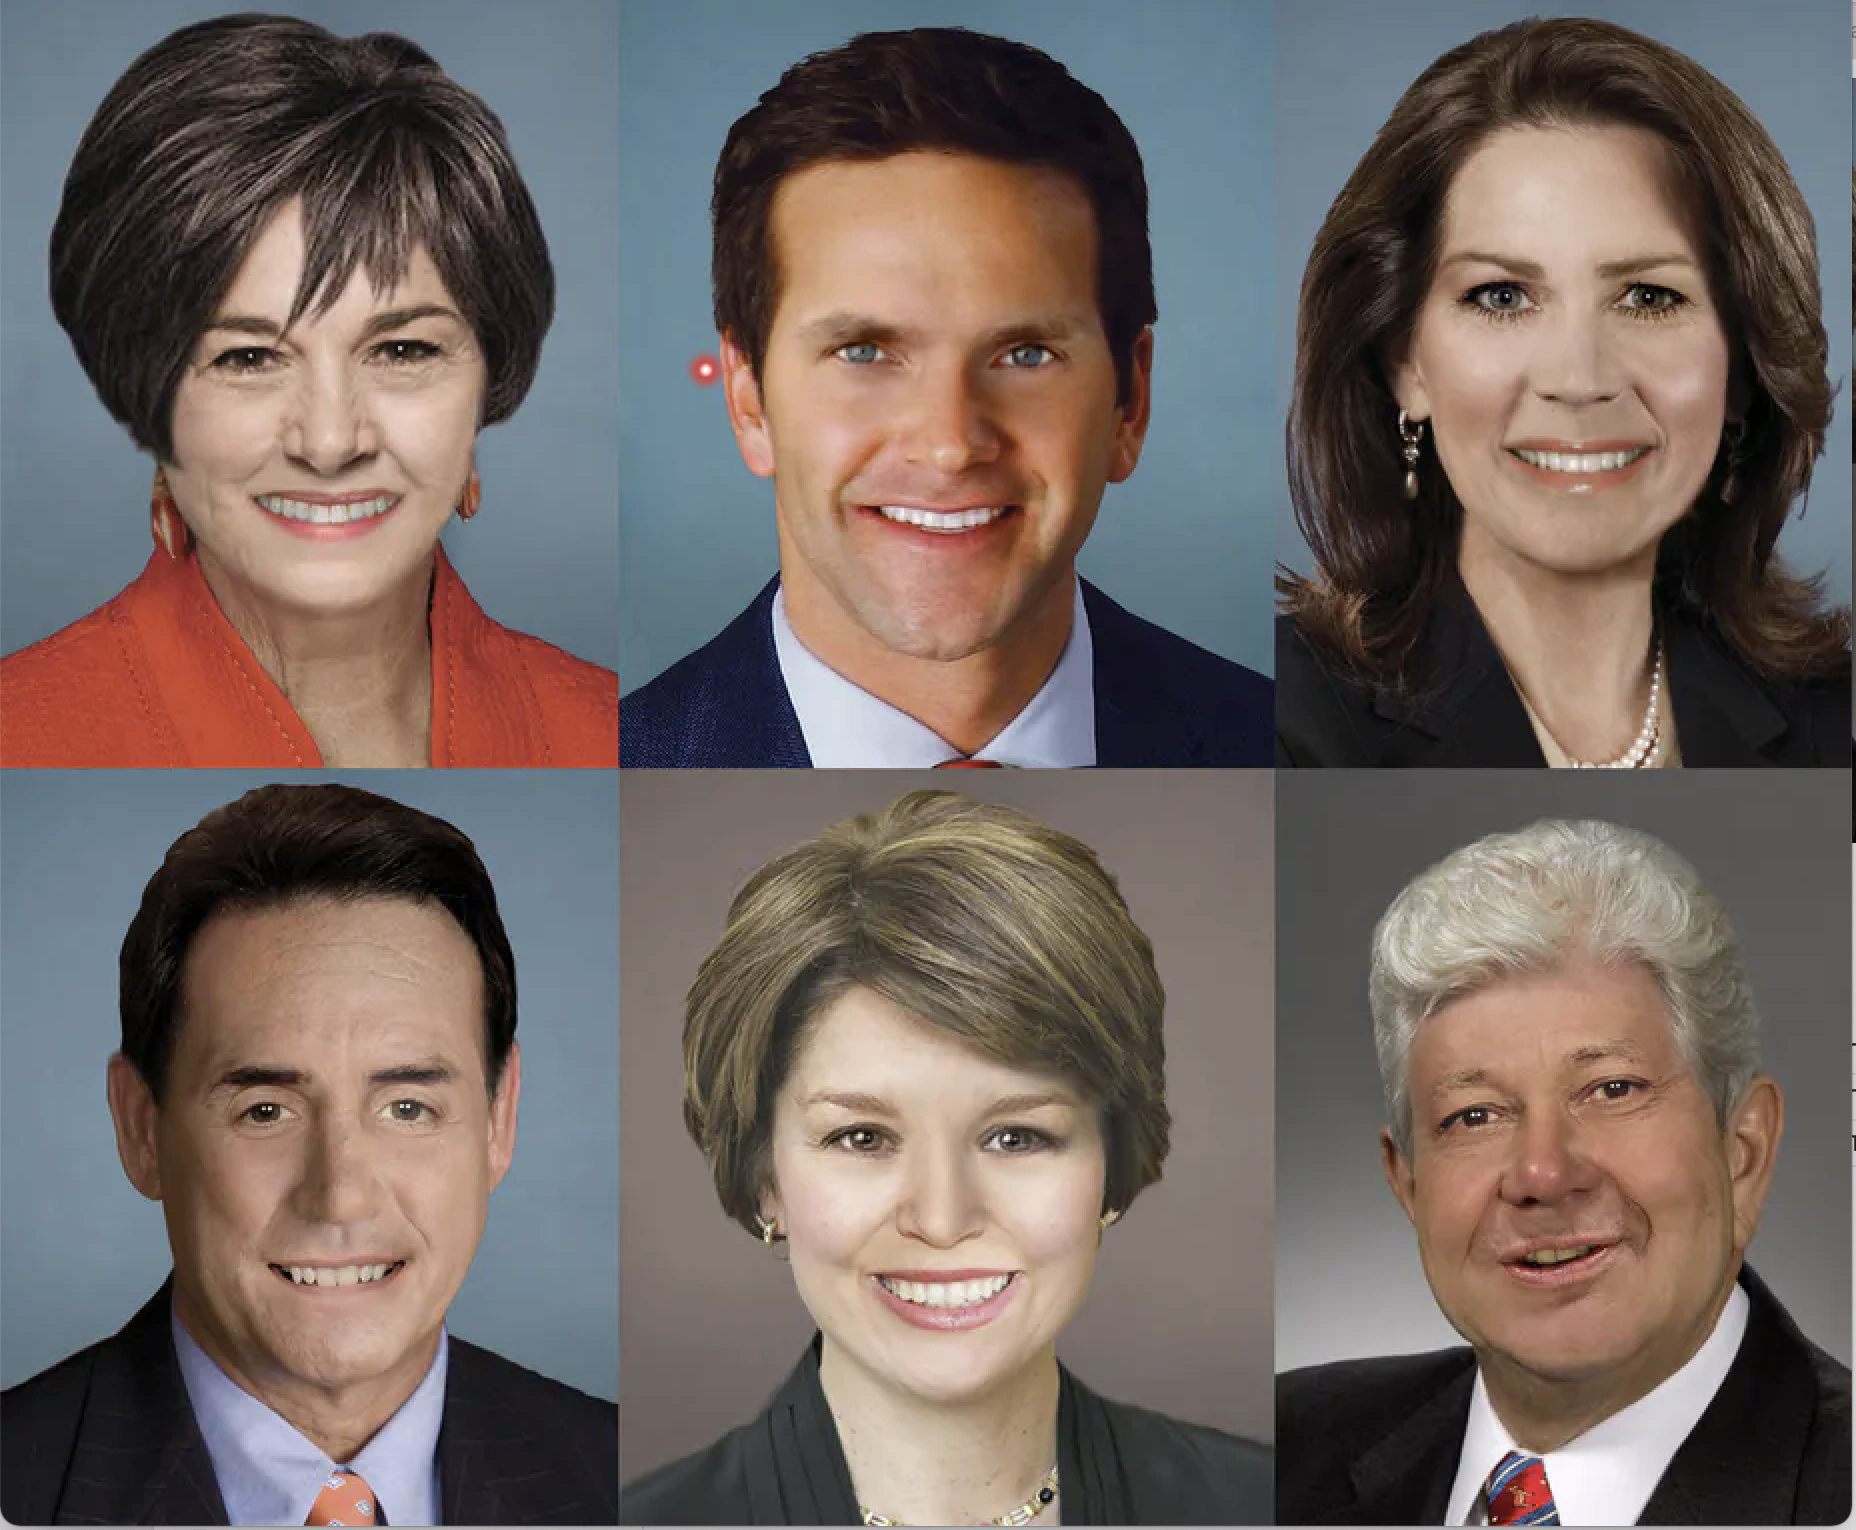
\includegraphics[width=\textwidth]{pic_4.png}
{\tiny ``What Are Good-Looking Candidates?'' (Stockemer and Praino, 2019)}
\end{column}
\end{columns}
\end{frame} 



% 1
\miniframesoff
\begin{frame}[c]{Nixon-Kennedy 1960 Debate}
\begin{columns}
\begin{column}{.45\textwidth}
\begin{itemize}
  \item Nixon's ``five-o'clock'' shadow largely affected voter evaluations.\\{\tiny \color{gray}Mattes et. al (2010).}
  \item[] {\color{white}Nixon didn't look right.}
  \item[] {\color{white}And was all sweaty. {\tiny\color{white} Stockemer and Praino (2019)}.}
  \item[] {\color{white}Radio listeners thought Nixon would win, while TV-watchers though Kennedy would.}
\end{itemize}
\end{column}
\begin{column}{.45\textwidth}
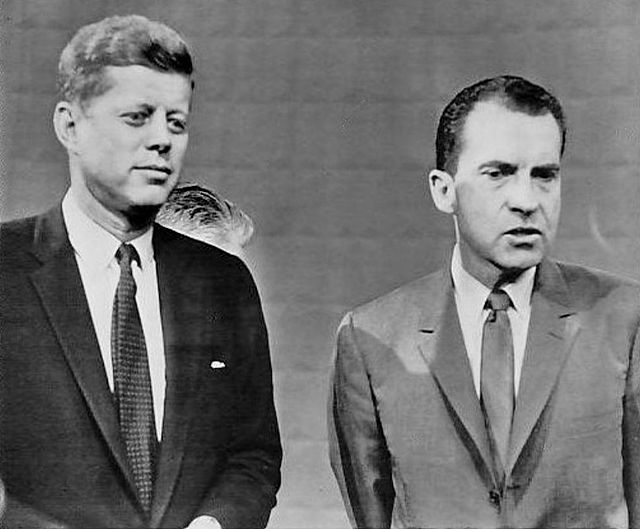
\includegraphics[width=\textwidth]{pic_1.jpg}
\end{column}
\end{columns}
\end{frame} 

% 2
\miniframesoff
\begin{frame}[c]{Nixon-Kennedy 1960 Debate}
\begin{columns}
\begin{column}{.45\textwidth}
\begin{itemize}
  \item Nixon's ``five-o'clock'' shadow largely affected voter evaluations.\\{\tiny\color{gray} Mattes et. al (2010).}
  \item Nixon didn't look right.
  \item[] {\color{white}And was all sweaty. {\tiny\color{white} Stockemer and Praino (2019).}}
  \item[] {\color{white}Radio listeners thought Nixon would win, while TV-watchers though Kennedy would.}
\end{itemize}
\end{column}
\begin{column}{.45\textwidth}
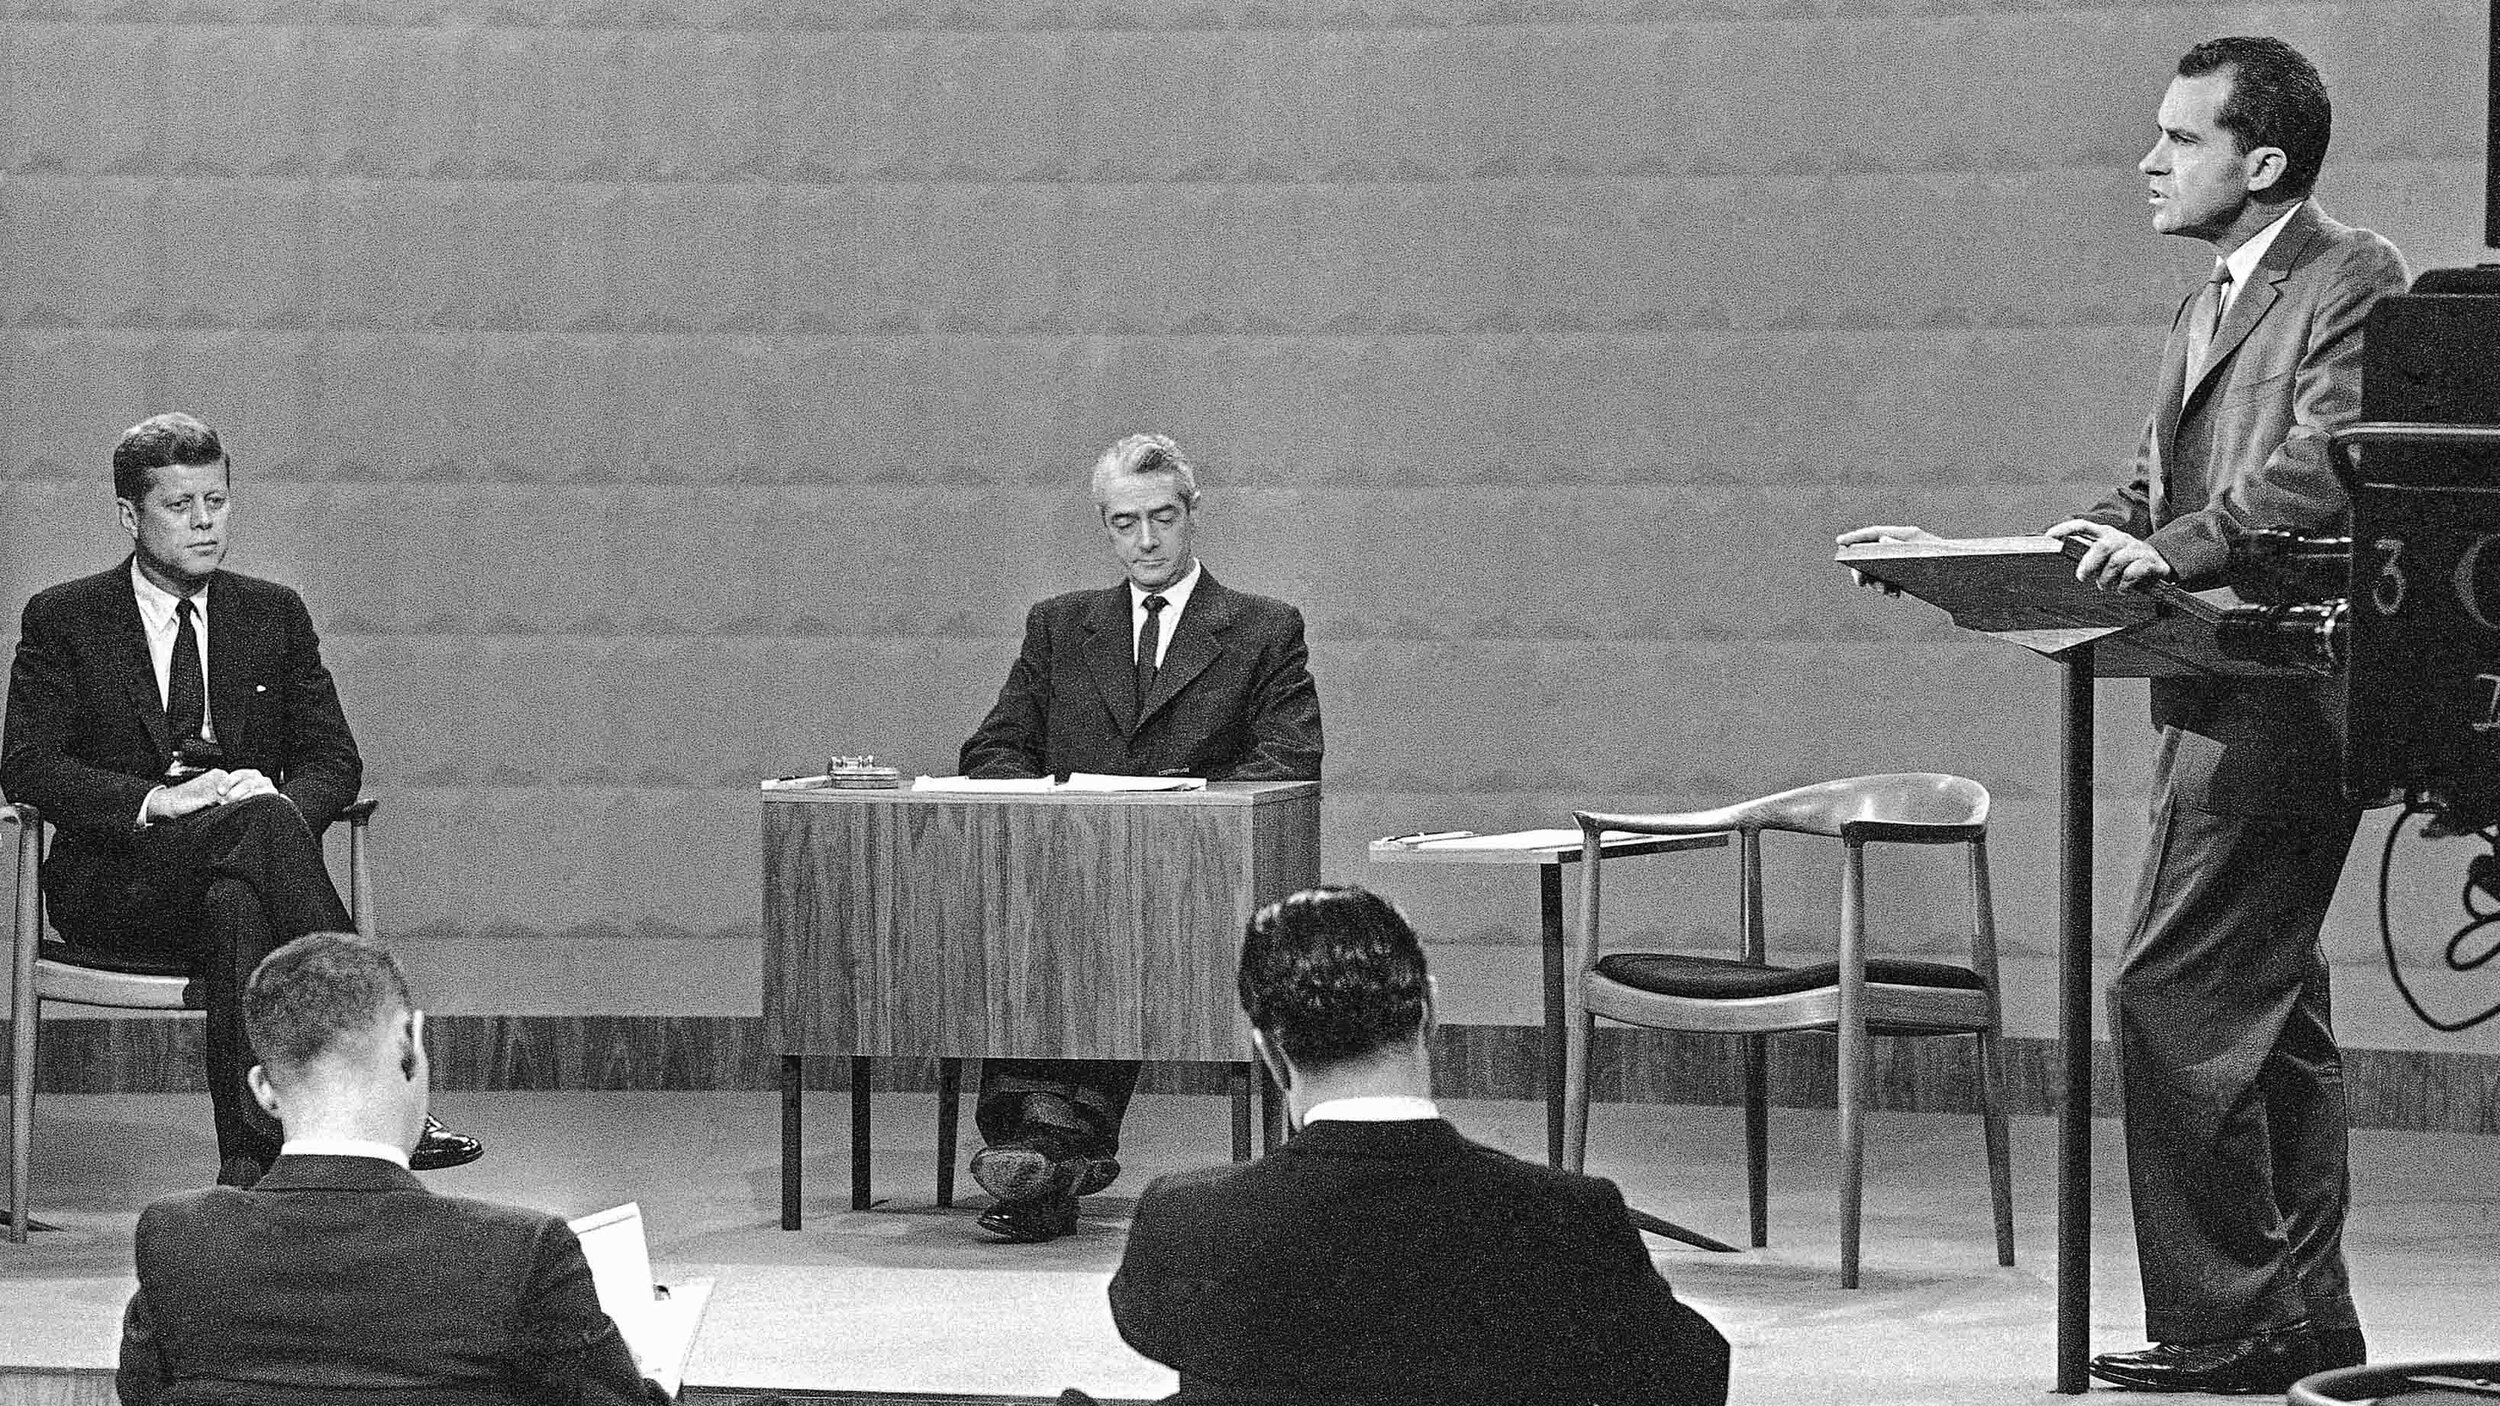
\includegraphics[width=\textwidth]{pic_2.JPG}
\end{column}
\end{columns}
\end{frame} 


% 3
\miniframesoff
\begin{frame}[c]{Nixon-Kennedy 1960 Debate}
\begin{columns}
\begin{column}{.45\textwidth}
\begin{itemize}
  \item Nixon's ``five-o'clock'' shadow largely affected voter evaluations.\\{\tiny \color{gray} Mattes et. al (2010).}
  \item Nixon didn't look right.
  \item And was all sweaty.\\{\tiny\color{gray} Stockemer and Praino (2019).}
  \item[] {\color{white} Radio listeners thought Nixon would win, while TV-watchers though Kennedy would.}
\end{itemize}
\end{column}
\begin{column}{.45\textwidth}
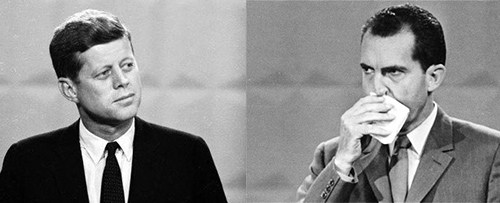
\includegraphics[width=\textwidth]{pic_3.jpg}
\end{column}
\end{columns}
\end{frame} 

% 4
\miniframesoff
\begin{frame}[c]{Nixon-Kennedy 1960 Debate}
\begin{columns}
\begin{column}{.45\textwidth}
\begin{itemize}
  \item Nixon's ``five-o'clock'' shadow largely affected voter evaluations.\\{\tiny \color{gray} Mattes et. al (2010).}
  \item Nixon didn't look right.
  \item And was all sweaty.\\{\tiny\color{gray} Stockemer and Praino (2019).}
  \item Radio listeners thought Nixon would win, while TV-watchers though Kennedy would.
\end{itemize}
\end{column}
\begin{column}{.45\textwidth}
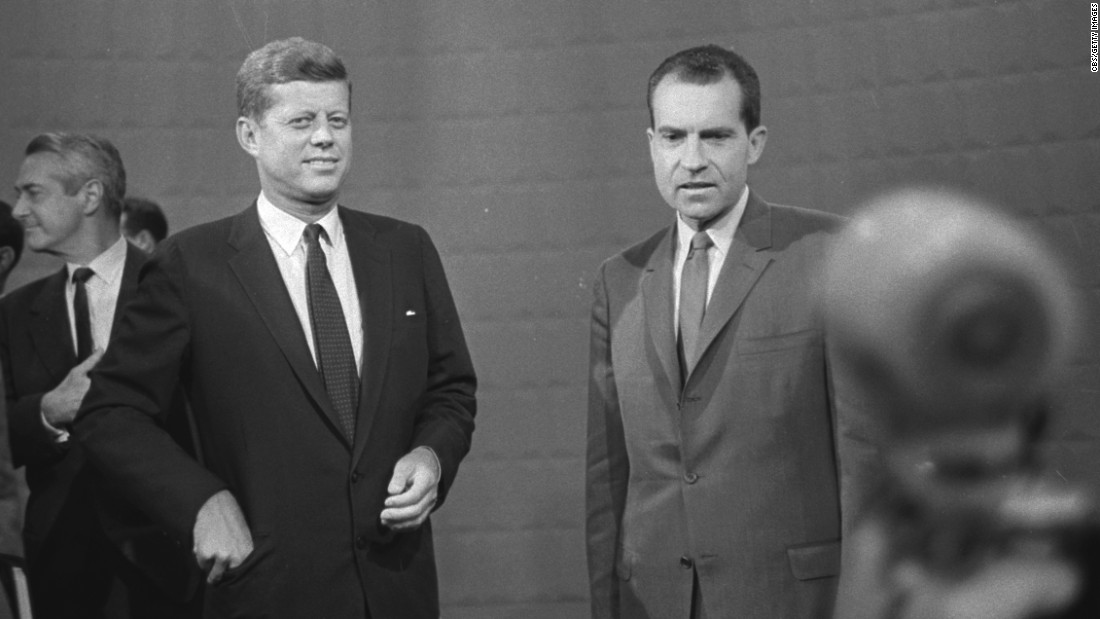
\includegraphics[width=\textwidth]{pic_5.jpg}
\end{column}
\end{columns}
\end{frame} 


\subsection{Gaps}


\miniframeson
\begin{frame}[c]{Gaps in the Current Literature}
\begin{itemize}
  \item While the literature has advanced a number of important questions, its focus has been on just {\bf attractiveness}.
  \item We believe that physical \emph{appearance} goes way beyond \emph{attractiveness}.
  \item Even while some have studied how ``looking \emph{competent}'' (and not necessarily ``\emph{beautiful}'') helps candidates winning elections, there are a number of unanswered questions.
  \item Importantly, several of these questions are related to inequality.
  \item {\bf In this paper we want to explain {\color{red}turnout}}: {\color{blue}\emph{Does it matter if the candidate look like a working-class individual as opposed to a white-collar individual?}}
\end{itemize}
\end{frame} 


\subsection{Filling in the Gaps}


\miniframeson
\begin{frame}[c]{To Fill These Gaps...}
\begin{itemize}
  \item Study the electoral consequences for candidates of {\bf looking} ``upper-class,'' ``middle-class'' or ``working-class.''
  \item Exploit a {\bf novel data} set were we are able to measure different physical appearance aspects of a subsample of political candidates.
  \item {\bf Find} that Finns vote systematically more for ``upper-class'' candidates, but that there are important gender differences.
\end{itemize}
\end{frame} 



\section{Theory}

\subsection{Political Psychology and Heuristics}

\miniframeson
\begin{frame}[c]{Political Psychology}
    \begin{itemize}
      \item A candidate's {\bf physical appearance} is ``the most important'' {\color{gray}\tiny (Lau \& Redlawsk 2001)} and the ``most obvious and accessible'' {\color{gray}\tiny (Dion et al. 1972)} \emph{heuristic} available to voters {\color{gray}\tiny (Stockemer \& Praino 2017)}.

      \item {\bf Heuristics} are cognitive devices that allow reasonable voting decision making with minimal effort {\color{gray}\tiny (Lau \& Redlawsk 2001 and Tversky \& Kahneman 1973)}.

      \item Thus, ``{\color{blue}voters vote beautiful}'' {\color{gray}\tiny(Efrain \& Patterson 1974)} because attractive candidates ``are more likely to be attributed the {\color{blue}qualities} associated with {\color{blue}successful} politicians'' {\color{gray}\tiny(Stockemer \& Praino 2019)}.

    \end{itemize}
\end{frame}



\subsection{Expectation States Theory and Inequality}

\miniframeson
\begin{frame}[c]{Expectation States Theory}
    \begin{itemize}
      \item {\bf Expectation States Theory}: physical appearance, gender and occupation ``cue social categories and signify social status'' making them all a ``locus of inequality.''

      - ``sexual attractiveness'' is a gender-specific status symbol: physical attractiveness intersects with gender producing unfavorable outcomes for women.


    \end{itemize}
\end{frame}


\section{Argument}

\subsection{Argument}


\miniframeson
\begin{frame}<presentation:0>
    \begin{enumerate}

      \item Differences between social groups (gender, occupation, race, etc.) are translated into social inequalities.

      \item For instance, women are more likely to get penalized because of how they look.

      \item In the context of low-information elections, a candidate with a lower status is faced with lower performance expectation, that is, lower turnout. 

      \item Since voters use heuristics, they will elect more systematically high-status male candidates than similar female candidates.

    \end{enumerate}
\end{frame}


\miniframeson
\begin{frame}[c]%{Argument}
\centering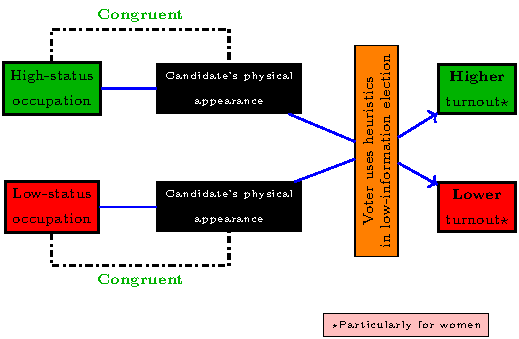
\includegraphics[scale=1.2]{argument.pdf}
\end{frame}

\section{Empirics}

\subsection{Case}

\miniframeson
\begin{frame}[c]{Finland as a Hard Case}
  \begin{itemize}
    \item We follow a ``{\bf least-likely case design}'' {\color{gray}\tiny(Levy 2008).} Finland has been consistently considered as:
      \begin{itemize}
        \item[-] A democratic {\color{gray}\tiny (Polity-V)}.
        \item[-] An economic egalitarian {\color{gray}\tiny (Waltl 2022)}.
        \item[-] A gender egalitarian.
        \item[-] A social-mobility prone country {\color{gray}\tiny (Erola 2009)}.
        %\item[-] Having low-information Municipal Elections {\color{gray}\tiny(Berggren et al. 2010 and 2017)}.
      \end{itemize}
      \item Thus, it should be {\bf hard to find} a correlation between class-congruent use of status symbols and turnout.
    \end{itemize}
\vspace{0.5cm}
{\color{gray}...and yet, we \emph{do}.}
\end{frame}

\miniframesoff
\begin{frame}[c]{Municipal Elections in Finland}
  \begin{itemize}
    \item {\bf Municipal Elections}: held every four years to elect councilors of the different municipalities {\color{gray}(N=293)}.
    \item {\bf D'Hondt}: candidates run in party lists. Sits are filled with lists of candidates proportionally.
    \item {\bf Municipalities}: provide daycare, health, education, water, waste management, among others.
  \end{itemize}
\end{frame}

\miniframesoff
\begin{frame}[c]{Campaigns: Plain, Simple and Fair}
\begin{columns}
\begin{column}{.45\textwidth}
\begin{itemize}
  \item {\bf ``Low-information'' elections}: most voters get exposed to only the official candidate pictures shown in the posters.\\
  {\color{gray}\tiny(Berggren et al. 2010 \& 2017).}
  \item {\bf Public information}: shown in city centers, bus stops, \emph{and} voting booths!
  \item Municipalities \emph{must} provide the \emph{same} number of poster slots for all parties.
\end{itemize}
\end{column}
\begin{column}{.45\textwidth}
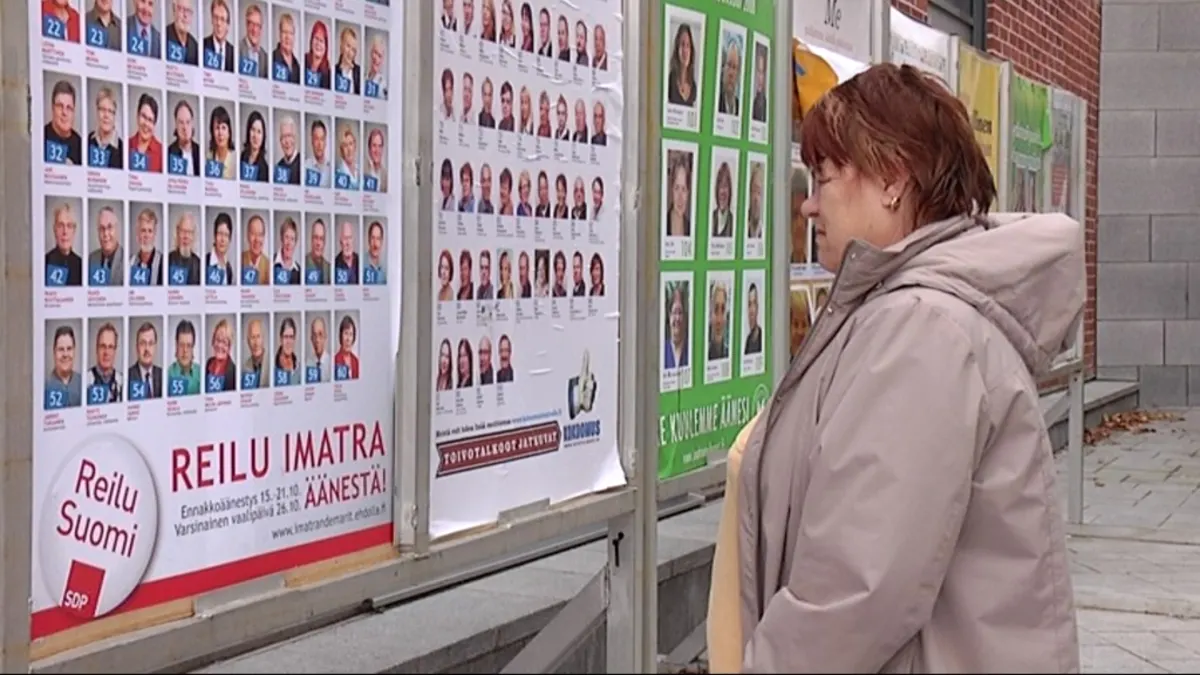
\includegraphics[width=\textwidth]{campaign2.png}
{\tiny Average Poster Displaying Candidates Faces in Finnish Elections}
\end{column}
\end{columns}
\end{frame} 



\subsection{Data}

\miniframeson
\begin{frame}[c]{2017 Municipal Elections: Candidate Data}
  \begin{itemize}
    \item {\bf Ministry of Justice}: candidate's pictures, district, occupation and turnout.
    \item {\bf Sample}: Universe 33,618, possible 10,000, randomly selected {\bf 1,500 candidate photographs}. 
    \item {\bf Occupation}: {\color{blue}European Socio-economic Classification}, recoded each candidate's occupation (upper, middle and working class).
  \end{itemize}
\end{frame}


\miniframesoff
\begin{frame}[c]{Novel Raters Data}
  \begin{itemize}
    \item {\bf Sample}: able to collect data from 7,920 randomly selected Finnish-speaking Finns.
    \item {\bf Task}: participants evaluated a random sample of candidate photographs according to five items (N$\sim$50).
    \item {\bf Items}: 
      \begin{enumerate}
        \item {\bf \scriptsize Occupation-Congruent Appearance}.
        \item {\bf \scriptsize Attractiveness}.
        \item {\bf \scriptsize Masculinity}.
        \item {\bf \scriptsize Femininity}.
      \end{enumerate}
    \item {\bf Avoiding recognition}: proprietary software designed to avoid assigning candidates running in the same district of the rater's.
     
  \end{itemize}
   \hyperlink{table:items}{\beamergotobutton{show table with items}}
\end{frame}

\miniframesoff
\begin{frame}[plain]%{Argument}
\centering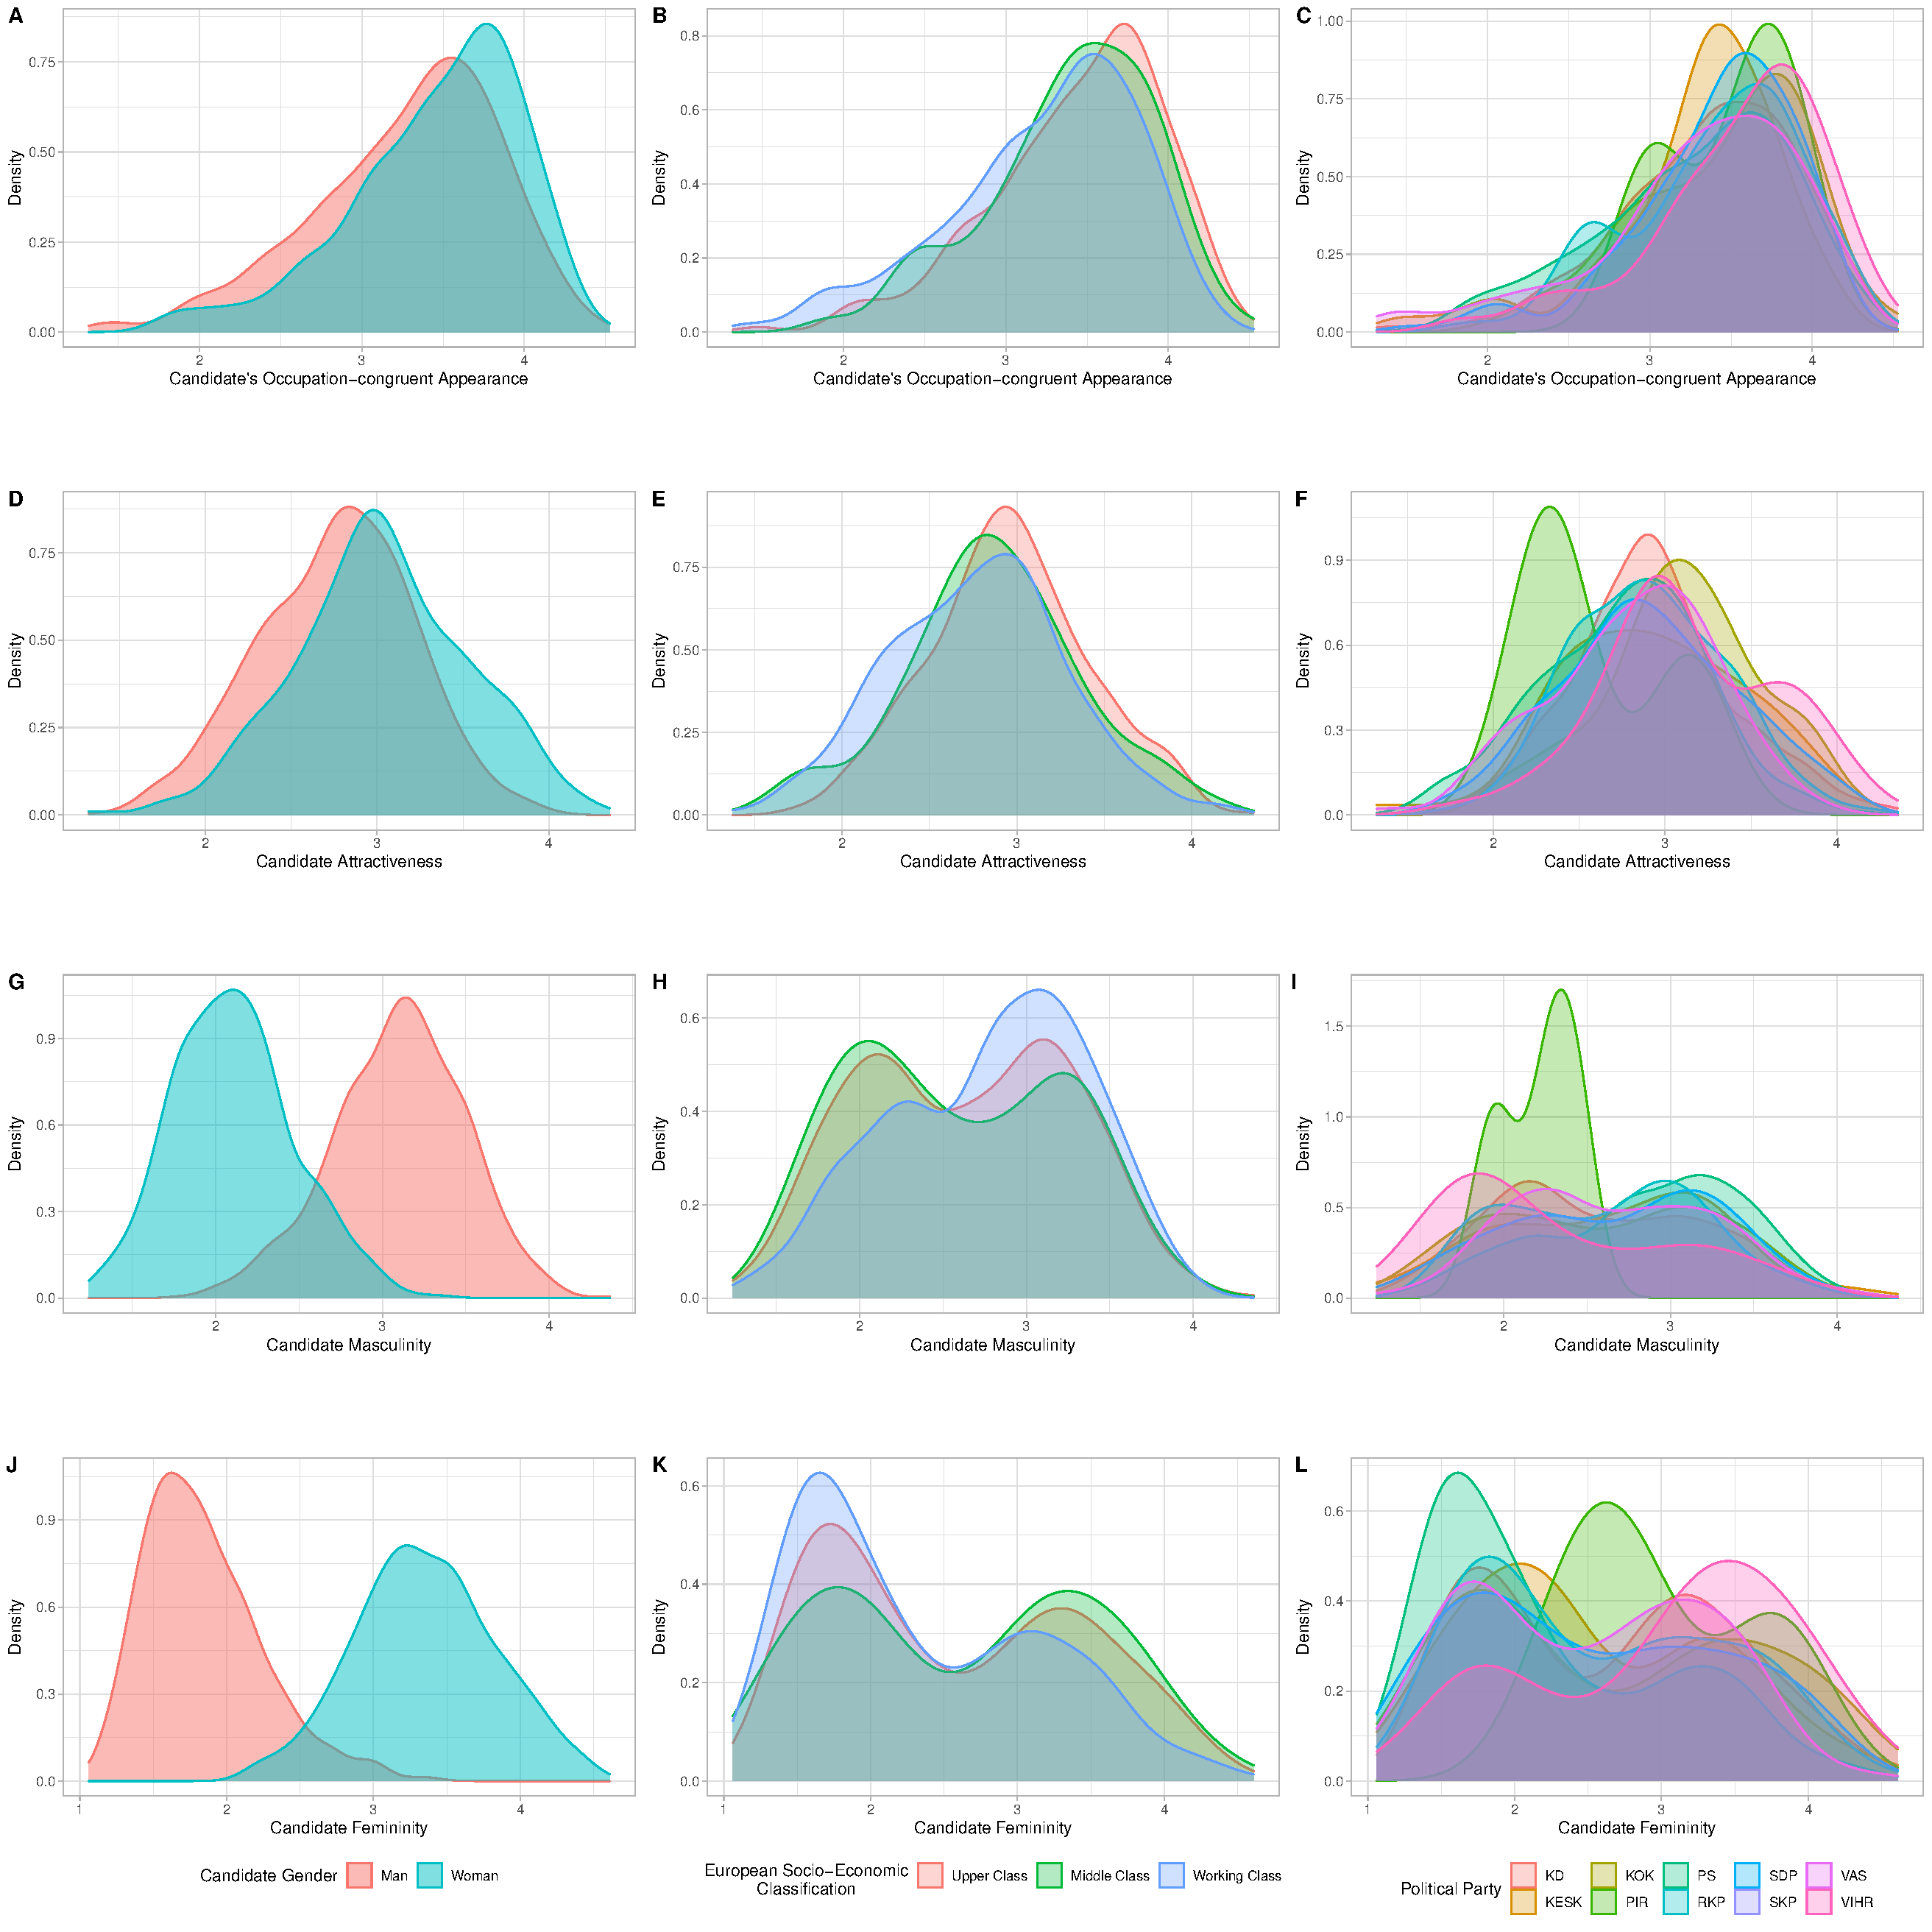
\includegraphics[scale=0.1999]{densities.pdf}
\end{frame}


\subsection{Statistical Analyses}


\miniframeson
\begin{frame}[c]{Functional Form and Model}

 \begin{align*}
 Y_{i}=\text{Turnout}_{i}\sim\;&\text{\texttt{Poisson}}\\
 \text{Turnout}_{i}  = \;
 & \beta_{0} + \\
 & \beta_{1}\text{{\only<2>{\color{red}}Occupation-congruent Appearance}}\times\text{{\only<2>{\color{red}}Social Class}} + \\
 & \beta_{2}\text{{\only<3>{\color{red}}Age}} + \\
 & \gamma{1}\text{{\only<4>{\color{red}}Party}} + \\
 & \gamma{2}\text{{\only<5>{\color{red}}City}}
 \end{align*}
 \begin{itemize}
  \item {\bf Also control for}: {\only<6>{\color{red}}Attractiveness}, {\only<7>{\color{red}}Masculinity} and {\only<8>{\color{red}}Femininity}.
 \item {\bf Partition the data} ({\only<9>{\color{red}}full}, {\only<10>{\color{red}}men} \& {\only<11>{\color{red}}women}).
\end{itemize}
\end{frame}


\miniframesoff
\begin{frame}[plain]%{Functional Form and Model}
\center

\begin{table}[H]
\caption{Statistical Models}
\begin{center}
\scalebox{0.4}{
\begin{threeparttable}
\begin{tabular}{l c c c c c c c c c c c c}
\hline
 & \multicolumn{1}{c}{1} & \multicolumn{1}{c}{2} & \multicolumn{1}{c}{3} & \multicolumn{1}{c}{4} & \multicolumn{1}{c}{5} & \multicolumn{1}{c}{6} & \multicolumn{1}{c}{7} & \multicolumn{1}{c}{8} & \multicolumn{1}{c}{9} & \multicolumn{1}{c}{10} & \multicolumn{1}{c}{11} & \multicolumn{1}{c}{12} \\
\cline{2-2} \cline{3-3} \cline{4-4} \cline{5-5} \cline{6-6} \cline{7-7} \cline{8-8} \cline{9-9} \cline{10-10} \cline{11-11} \cline{12-12} \cline{13-13}
 & Full & Men & Women & Full & Full & Full & Men & Women & Men & Women & Men & Women \\
\hline
Intercept                                            & $4.49^{***}$  & $2.58^{***}$  & $6.17^{***}$  & $2.11^{***}$  & $4.27^{***}$  & $2.15^{***}$  & $-0.25^{**}$  & $3.24^{***}$  & $2.50^{***}$  & $2.98^{***}$  & $0.17$        & $2.80^{***}$  \\
                                                     & $(0.05)$      & $(0.08)$      & $(0.07)$      & $(0.05)$      & $(0.05)$      & $(0.05)$      & $(0.09)$      & $(0.08)$      & $(0.08)$      & $(0.08)$      & $(0.09)$      & $(0.08)$      \\
Physical Occupation-Congruent                        & $0.41^{***}$  & $0.59^{***}$  & $0.28^{***}$  & $0.25^{***}$  & $0.42^{***}$  & $0.26^{***}$  & $0.37^{***}$  & $0.22^{***}$  & $0.59^{***}$  & $0.28^{***}$  & $0.37^{***}$  & $0.24^{***}$  \\
                                                     & $(0.01)$      & $(0.01)$      & $(0.01)$      & $(0.01)$      & $(0.01)$      & $(0.01)$      & $(0.01)$      & $(0.01)$      & $(0.01)$      & $(0.01)$      & $(0.01)$      & $(0.01)$      \\
Middle Class                                         & $0.30^{***}$  & $0.81^{***}$  & $-0.05$       & $0.41^{***}$  & $0.23^{***}$  & $0.31^{***}$  & $0.54^{***}$  & $0.12$        & $0.77^{***}$  & $0.18$        & $0.75^{***}$  & $0.16$        \\
                                                     & $(0.06)$      & $(0.08)$      & $(0.11)$      & $(0.06)$      & $(0.06)$      & $(0.06)$      & $(0.08)$      & $(0.11)$      & $(0.08)$      & $(0.11)$      & $(0.08)$      & $(0.11)$      \\
Working Class                                        & $1.03^{***}$  & $1.59^{***}$  & $0.70^{***}$  & $0.49^{***}$  & $1.07^{***}$  & $0.58^{***}$  & $0.95^{***}$  & $0.23^{***}$  & $1.59^{***}$  & $0.32^{***}$  & $0.86^{***}$  & $0.19^{**}$   \\
                                                     & $(0.03)$      & $(0.04)$      & $(0.07)$      & $(0.03)$      & $(0.03)$      & $(0.03)$      & $(0.04)$      & $(0.07)$      & $(0.04)$      & $(0.07)$      & $(0.04)$      & $(0.07)$      \\
Age                                                  & $-0.02^{***}$ & $-0.01^{***}$ & $-0.03^{***}$ & $-0.00^{***}$ & $-0.02^{***}$ & $-0.01^{***}$ & $0.00^{***}$  & $-0.01^{***}$ & $-0.01^{***}$ & $-0.02^{***}$ & $0.01^{***}$  & $-0.01^{***}$ \\
                                                     & $(0.00)$      & $(0.00)$      & $(0.00)$      & $(0.00)$      & $(0.00)$      & $(0.00)$      & $(0.00)$      & $(0.00)$      & $(0.00)$      & $(0.00)$      & $(0.00)$      & $(0.00)$      \\
Physical Occupation-Congruent $\times$ Middle Class  & $-0.18^{***}$ & $-0.34^{***}$ & $-0.11^{***}$ & $-0.20^{***}$ & $-0.16^{***}$ & $-0.17^{***}$ & $-0.22^{***}$ & $-0.17^{***}$ & $-0.33^{***}$ & $-0.19^{***}$ & $-0.28^{***}$ & $-0.18^{***}$ \\
                                                     & $(0.02)$      & $(0.02)$      & $(0.03)$      & $(0.02)$      & $(0.02)$      & $(0.02)$      & $(0.02)$      & $(0.03)$      & $(0.02)$      & $(0.03)$      & $(0.02)$      & $(0.03)$      \\
Physical Occupation-Congruent $\times$ Working Class & $-0.46^{***}$ & $-0.61^{***}$ & $-0.43^{***}$ & $-0.28^{***}$ & $-0.48^{***}$ & $-0.31^{***}$ & $-0.39^{***}$ & $-0.28^{***}$ & $-0.62^{***}$ & $-0.29^{***}$ & $-0.35^{***}$ & $-0.27^{***}$ \\
                                                     & $(0.01)$      & $(0.01)$      & $(0.02)$      & $(0.01)$      & $(0.01)$      & $(0.01)$      & $(0.01)$      & $(0.02)$      & $(0.01)$      & $(0.02)$      & $(0.01)$      & $(0.02)$      \\
Attractiveness                                       &               &               &               & $0.76^{***}$  &               & $0.89^{***}$  & $1.00^{***}$  & $0.72^{***}$  &               &               & $1.08^{***}$  & $0.53^{***}$  \\
                                                     &               &               &               & $(0.01)$      &               & $(0.01)$      & $(0.01)$      & $(0.01)$      &               &               & $(0.01)$      & $(0.01)$      \\
Masculinity                                          &               &               &               &               & $0.09^{***}$  &               &               &               & $0.04^{***}$  &               & $-0.28^{***}$ &               \\
                                                     &               &               &               &               & $(0.00)$      &               &               &               & $(0.01)$      &               & $(0.01)$      &               \\
Femininity                                           &               &               &               &               &               & $-0.15^{***}$ &               &               &               & $0.68^{***}$  &               & $0.26^{***}$  \\
                                                     &               &               &               &               &               & $(0.00)$      &               &               &               & $(0.01)$      &               & $(0.02)$      \\
\hline
AIC                                                  & $287653.94$   & $170596.79$   & $79111.45$    & $267973.43$   & $287029.77$   & $265328.79$   & $154959.12$   & $73290.19$    & $170577.24$   & $74331.79$    & $153861.01$   & $73001.39$    \\
BIC                                                  & $288886.12$   & $171561.82$   & $79936.45$    & $269210.66$   & $288267.17$   & $266571.24$   & $155928.83$   & $74119.20$    & $171546.96$   & $75161.13$    & $154835.41$   & $73834.74$    \\
Log Likelihood                                       & $-143590.97$  & $-85092.40$   & $-39365.73$   & $-133749.72$  & $-143277.88$  & $-132426.40$  & $-77272.56$   & $-36454.09$   & $-85081.62$   & $-36974.89$   & $-76722.51$   & $-36308.70$   \\
Deviance                                             & $278666.41$   & $165250.11$   & $75150.60$    & $258990.24$   & $278040.23$   & $256343.60$   & $149610.43$   & $69333.68$    & $165228.56$   & $70368.94$    & $148510.33$   & $69042.88$    \\
Num. obs.                                            & $1368$        & $800$         & $568$         & $1367$        & $1368$        & $1367$        & $800$         & $567$         & $800$         & $568$         & $800$         & $567$         \\
\hline
\end{tabular}
\begin{tablenotes}[flushleft]
\scriptsize{\item $^{***}p<0.001$; $^{**}p<0.01$; $^{*}p<0.05$. \item Dependent variable is Turnout. City fixed effects and party variables omitted. The reference category in the ESEC variable is 'Upper Class.' Given the symmetry of the derivatives, changing the reference category does not alter the interpretation of the results. Functional form is Poisson regression for all models.}
\end{tablenotes}
\end{threeparttable}
}
\label{reg:t}
\end{center}
\end{table}

\end{frame}


\miniframesoff
\begin{frame}[c]{Main Results}
\centering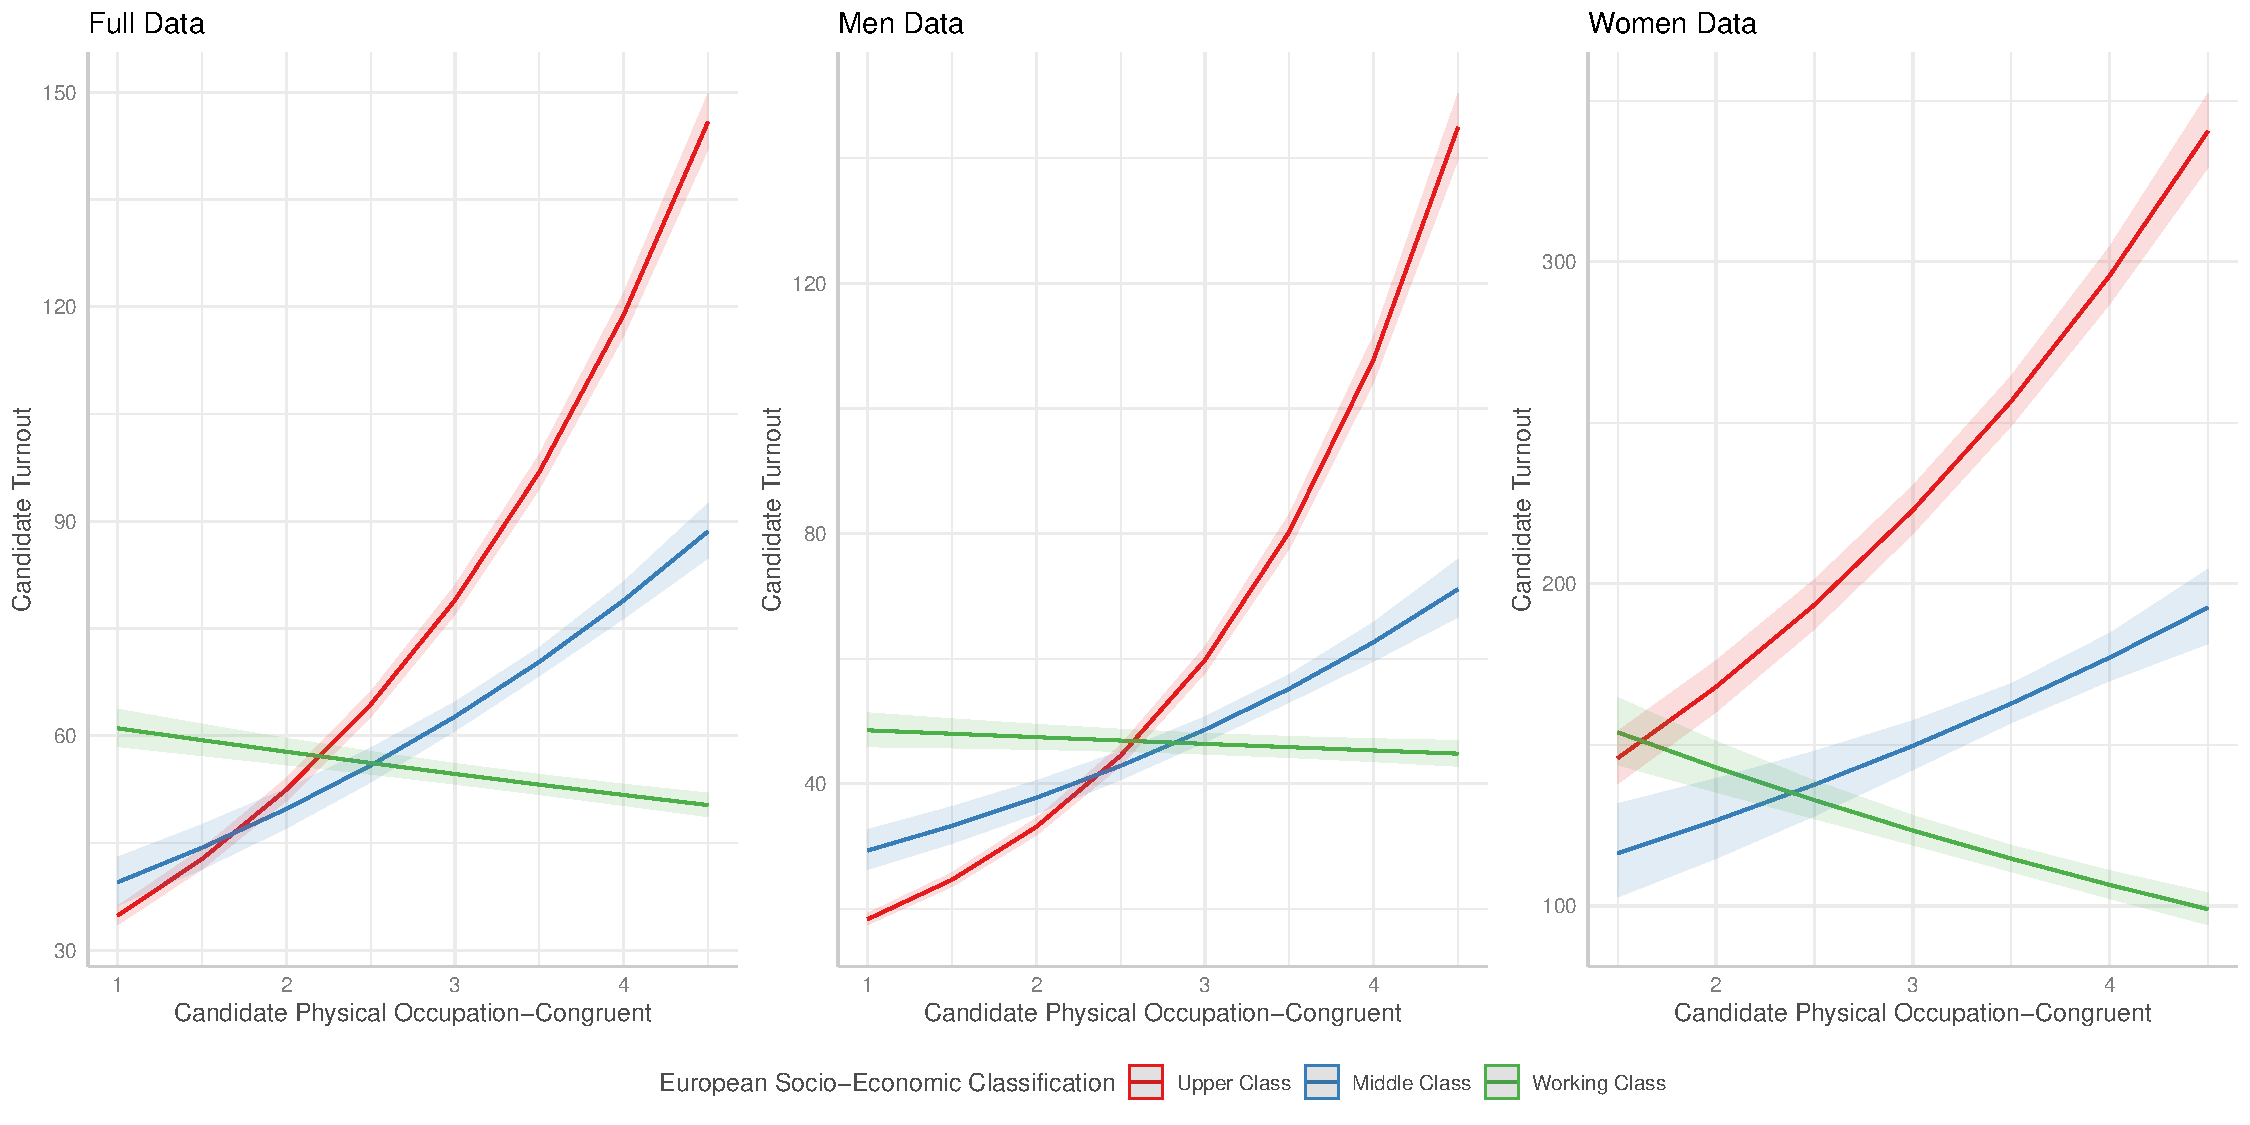
\includegraphics[scale=0.3]{pred_prob_plot.pdf}
\end{frame}

\section{Discussion}

\subsection{At a Glance}

\miniframeson
\begin{frame}[c]{Main Results}
      \begin{itemize}
        \item {\bf Male \& female} candidates:  
          \begin{enumerate}
            \item[$\checkmark$] Candidates that show {\color{black!30!green}\emph{higher degrees of congruence}} between physical appearance and occupation {\color{black!30!green}do better}.
            \item[$\checkmark$] Candidates that look-like and also perform {\color{black!30!green}\emph{upper-class occupations} do best} in elections.
          \end{enumerate}
        \item  {\bf Female} candidates: stronger effects.
          \begin{itemize}
          \item Systematic {\color{red}electoral penalty} when they {\color{red}{\bf look-like}} and also {\bf perform {\color{red}working-class} occupations}.
          \item Systematic {\color{black!30!green}electoral premium} when they {\color{black!30!green}{\bf look-like}} and also {\bf perform {\color{black!30!green}white-collar} occupations}.
        \end{itemize}
      \end{itemize}
\end{frame}

\subsection{Wrapping Up}

\miniframeson
\begin{frame}[c]{Main Takeaways}
  \begin{itemize}
    \item[$\checkmark$] Considered {\bf the use of heuristics in elections} and the concept of {\bf ``status'' in expectation states theory}.
    \item[$\checkmark$] Selected the {\bf \emph{unlikely} case} of the 2017 Finnish Municipal Elections.
    \item[$\checkmark$] Exploited a {\bf novel representative data set} on candidates physical appearances.
    \item[{\color{black!30!green}$\checkmark$}] Proposed an alternative explanation for {\color{red}turnout} not based on attractiveness but on {\color{black!30!green}occupation-congruent appearance} and {\color{black!30!green}social stratification}.
  \end{itemize}
\end{frame}

\miniframesoff
\begin{frame}[c]{Thank you}
        %\begin{center}
        %  \vspace{-0.7cm}\includegraphics[scale=.05, center]{/Users/hectorbahamonde/hbahamonde.github.io/resources/qr-code.pdf}
        %\end{center}


        \begin{itemize}
            %\item Paper (draft) available at {\color{blue}www.HectorBahamonde.com}.
            \item[] All feedback is welcomed!
        \end{itemize}
\end{frame}


%%%%%%%%%%%%%%%%%%%%%%%%%%%%%%%%
% APPENDIX
%%%%%%%%%%%%%%%%%%%%%%%%%%%%%%%%

\section{Appendix}

% Raters Data: Questions and Answer Set
\miniframesoff
\begin{frame}[c]{\hypertarget{table:items}{Raters Data: Questions and Answer Set}}
\begin{table}[h]\tiny
\begin{tabularx}{\textwidth}{|c||c|X|X|X}%{@{}l *3{>{\centering\arraybackslash}X}@{}}%{|c||cX|X|X}
{\bf Sample} & {\bf Attribute} & {\bf Question} & {\bf Answer Set} \\
\hline
1      & Occupation-Congruent Appearance & To what extent does this person respond to your image of someone working in [occupation]? & 5=Perfectly responds to my image, 4=Responds well to my image, 3=Somewhat responds to my image, 2=Does not respond to my image well, 1=Does not respond to my image at all. \\
\hline
2      & Attractiveness & In your opinion, how attractive does this person look, as compared to others of the same age and gender?   & 5=very attractive, 4=more attractive than the average, 3=average, 2=below average, 1=well below average (Griffin and Langois 2006; Bono et al. 2017; Tu, Gilbert and Bono 2021)\\
\hline
3      & Masculinity & To what extent do you think this person looks masculine, as compared to others of the same age and gender? & 1=not masculine at all, to 5=very masculine (e.g., Hoss et al. 2005).\\
\hline
4      & Femininity & To what extent do you think this person looks feminine, as compared to others of the same age and gender?  & 1=not feminine at all, to 5=very feminine.  
\end{tabularx}
\end{table}
\end{frame}




\end{document}



                                                                                                                                                                               
